\documentclass[12pt, letterpaper]{article}
\usepackage[utf8]{inputenc}
\usepackage[left = 2.5cm, right = 2.5cm, top = 2.5cm, bottom = 2.5cm]{geometry}
\usepackage{amsthm}
\usepackage{amsfonts}
\usepackage{amsmath}
\usepackage{amssymb}
\usepackage{graphicx}
\usepackage[T1]{fontenc}
\graphicspath{{images/}}



\author{Hernández Ferreiro Enrique Ehecatl \\
        López Soto Ramses Antonio \\
        Miguel Torres Eric Giovanni \\
        Quintero Villeda Erik}

\title{Práctica 3: Modelo Entidad-Relación \\
       {\small Fudamentos de Bases de Datos}}

\date{9 de septiembre de 2019}

\begin{document}
    \maketitle

    \subsection*{Objetivo}
    Modelar un caso prueba con el esquema entidad-relación visto en clase.

    \section*{Introducción}
    El modelo entidad-relación se trata de una herramienta útil que nos
    proporciona una visión conceptual para poder representar información
    del mundo real. \vspace{.3cm}

    Las principales características que posee son:
    
    \begin{itemize}
        \item Notación gŕafica.
        \item Una semántica bastante clara.
        \item Es intuitivo.
        \item Independiante.
    \end{itemize}

    El modelo E/R posee distintos componentes con los cuales podemos modelar como:

    \begin{itemize}
        \item Entidades, que se dividen en físicos y conceptuales.
        \item Atributos, que son simples/compuestos, llaves, derivados, 
              univaluados/multivaluados.
        \item Relaciones, que pueden ser M:M, 1:M 1:1; con participación total/parcial.
    \end{itemize}

    \section*{Desarrollo}

    Para el modelado del caso prueba se realizaron pequeñas reuniones de una hora
    como se muestra a continuación: \vspace{.3cm}
 
        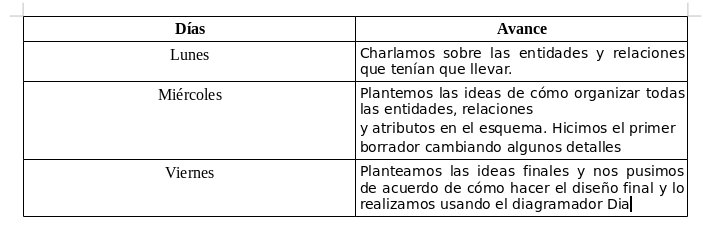
\includegraphics[scale=0.6]{tabla.png}
        
        El resultado obtenido de las reuniones es el siguiente: \vspace{.3cm}

        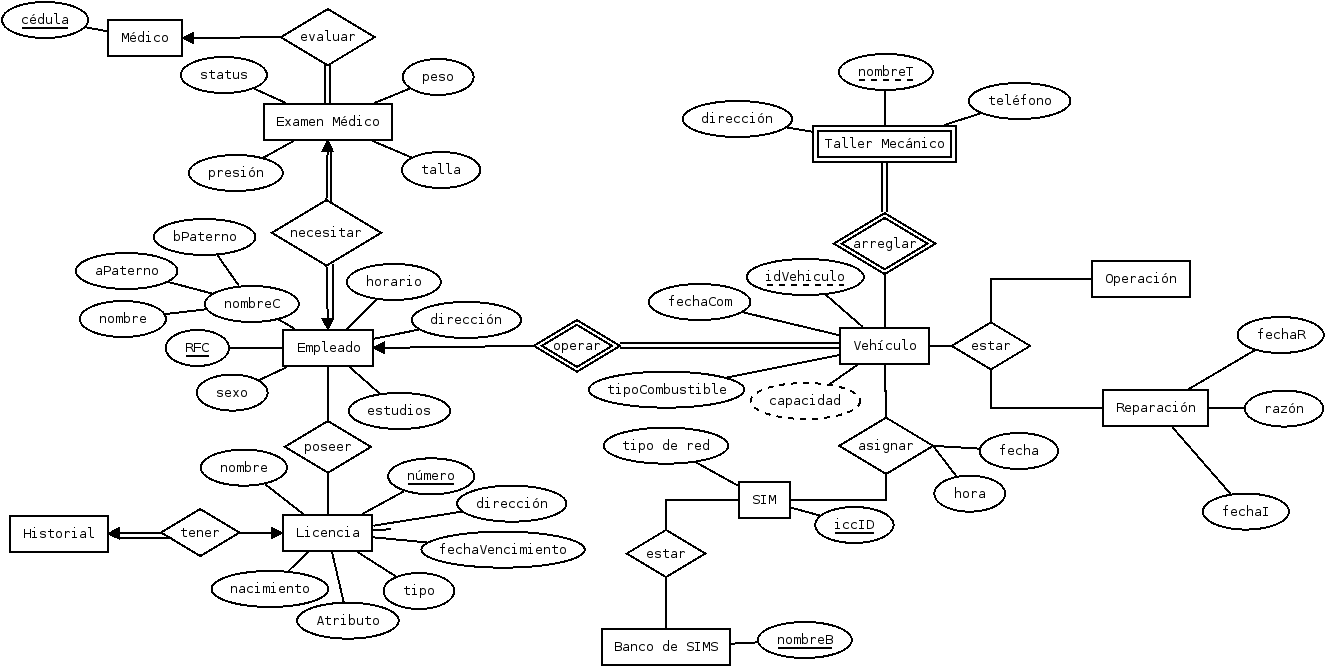
\includegraphics[scale=0.35]{practica3.png}
        
    \section*{Conclusión}
El diseño de cualquier problema a través de un modelo abstractacto como lo es el modelo E/R nos ayuda a tener una visión más clara de cómo
 se relacionan todas las entidades respetando ciertas restricciones.

\end{document}